Цель этапа составить два набора данных для обучения: параллельный корпус изображение-текст и наиболее полное описание задачи

\subsection{Разметка изображений}


В состав открытого тренировочного набора входит более десятка тысяч аннотированных изображений  
Результат моделирования предоставлены 
на открытых ресурсах\footnote{
\url{https://github.com/NMashalov/Generative-modeling-appliance-for-creating-educational-tasks}
и \url{https://huggingface.co/datasets/NMashalov/task_illustrations_dataset}
}

\subsubsection{Разметка}

Данные были собраны из открытых источников \cite{libmipt}\cite{mathedu}. 

\begin{figure}[h]
    \centering
    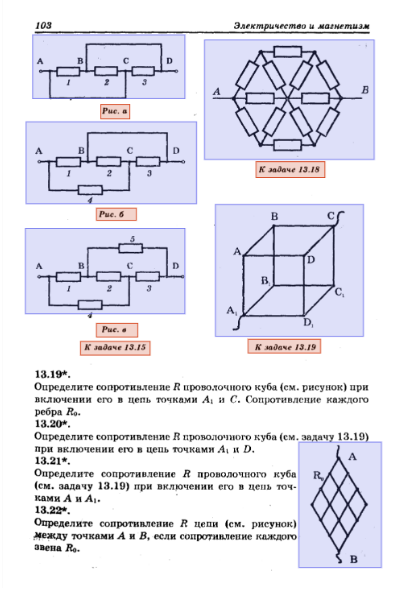
\includegraphics[width=0.5\textwidth]{assets/dataset/kirik_labeling.png}
    \caption{Пример аннотированной иллюстрации из книги Генденштейн, Кирик, Гельфгат: 1001 задача по физике}
    \label{annotation}
\end{figure}



Для получения обучающей выборки была проведена разметка части датасета. Каждое изображение включает в себя текстовую информацию, а также различные чертежи и формулы, характерные для данной области знаний.

Процесс разметки включал создание аннотаций для каждого изображения, а именно выделение границ объектов, таких как текстовые блоки, формулы и чертежи. Этот процесс требовал точности и внимательности для корректного определения границ объектов на изображении и их соответствия с аннотациями.

Для расширения датасета и обеспечения его разнообразия была применена аугментация данных. Применялись повороты, масштабирование, изменение освещения и отражение, позволили создать дополнительные вариации входных данных. 
Это способствовало увеличению разнообразия обучающей выборки и повышению устойчивости модели к различным вариациям данных, что важно для обеспечения ее эффективности в реальных условиях различной разметки страницы.


\subsubsection{Обучение нейросети для завершения разметки}


Для обучения на полученных данных была использована нейронная сеть YOLO. Эта архитектура нейронной сети имеет способность эффективно дообучаться на небольших выборках данных, что позволяет достигать удовлетворительных результатов.

Для ситуаций, где число аннотаций и число изображений на изображении не совпадало, применялся алгоритм на двудольном графе, направленный на максимизацию числа пар.


\subsection{Распознание текста}


Оптическое распознавание символов (OCR) представляет собой процесс автоматического преобразования текста, представленного в виде изображения или сканированного документа, в электронный текстовый формат. Термин "оптическое" в данном контексте указывает на использование оптических средств, таких как камеры или сканеры, для захвата изображений символов с физических носителей, например, бумаги.

Процесс OCR включает в себя несколько этапов, начиная с захвата изображения и заканчивая распознаванием символов и созданием электронного текста. Первоначально изображение документа подвергается предварительной обработке, такой как удаление шума или коррекция искажений. Затем происходит сегментация изображения, то есть разделение его на отдельные символы или группы символов.

Далее, при помощи алгоритмов распознавания, включающих методы машинного обучения и компьютерного зрения, символы на изображении анализируются и сопоставляются с соответствующими символами из набора знаков. Этот этап включает в себя распознавание формы символов, их контекста и других характеристик, что позволяет определить, какие символы были изображены на сканированном документе.

В завершение, распознанные символы объединяются в слова, предложения и абзацы, формируя полноценный текстовый документ. Точность и эффективность процесса OCR зависят от качества изображения, используемых алгоритмов распознавания, а также от языка и структуры текста. В современных приложениях OCR широко используются в различных областях, включая сканирование документов, распознавание номеров автомобильных номеров, оптическое чтение рукописных текстов и другие приложения, где требуется автоматическое извлечение текста из изображений.




